\documentclass{standalone}
\usepackage{tikz}
\usepackage{amsmath, amssymb}
\usetikzlibrary{automata, positioning}

\begin{document}
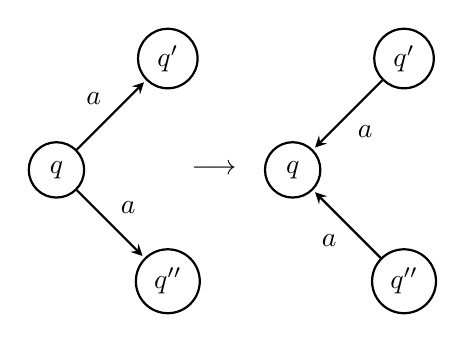
\begin{tikzpicture}[%
    >=stealth,
    shorten >=1pt,
    node distance=2cm,
    on grid,
    auto,
    state/.append style={minimum size=2em},
    thick
  ]

  \node[state] (A) {$q$};
  \node[state] (B) [above right of=A] {$q'$};
  \node[state] (C) [below right of=A] {$q''$};
  \node[state, draw=none] (Z) [right = 2cm of A] {$\longrightarrow$};
  \node[state] (E) [right= 1cm of Z]  {$q$};
  \node[state] (F) [above right of=E] {$q'$};
  \node[state] (G) [below right of=E] {$q''$};

  \path[->]
              (A)         edge [          ] node {$a$} (B)
              (A)         edge [          ] node {$a$} (C)
              (F)         edge [          ] node {$a$} (E)
              (G)         edge [          ] node {$a$} (E);
\end{tikzpicture}
\end{document}